\section{Analysis}
\vspace{-10pt}
In this section, we aim to delve into the factors influencing the performance of VLMs in digital agent tasks and their underlying behavioral logic. 
We will investigate the impact of task attributes (such as difficulty, feasibility, visual requirement, and GUI complexity), input measurements (such as screenshot resolution, the influence of trajectory history, and the effect of UI layout), explore whether there are patterns in the agent's performance across different operating systems, and make a qualitative analysis in the aspect of models, methods, and humans.
All experiments, unless specifically mentioned otherwise, are conducted using GPT-4V under the Set-of-Mark setting.
Some takeaways from the analysis are:
1) higher screenshot resolution typically leads to improved performance; 
2) encoding more a11y (text) trajectory history can boost performance, while not working for screenshots (image); 
3) current VLMs are not adept at image-based trajectory history context;
4) current VLM agents are not robust to UI layout and noise;
5) the performance of VLM agents across OS is in strong correlation;
6) VLM agents have common error types like mouse-clicking inaccuracies, limited domain knowledge, and more types discussed in Sec.~\ref{qualitative_analysis}.


\subsection{Performance by Task Difficulty, Feasibility and App Involved}
We analyze the success rate across several additional subsets of tasks, as summarized in Tab.~\ref{tab:task_subset} and will be discussed in the following sections.

\begin{wraptable}{r}{6cm}
\vspace{-15pt}
\caption{Success rate (SR) of GPT-4V (SoM) across different types of tasks.}
\centering
\resizebox{1.0\linewidth}{!}{%
\begin{tabular}{@{}lcc@{}}
\toprule
    Task Subset             & \% of Total & SR (↑) \\ \midrule
    Easy            & 28.72\%      & \textbf{16.78\%} \\
    Medium       & 40.11\%      & 13.12\% \\
    Hard        & 30.17\%      & 4.59\% \\
    \midrule
    Infeasible    & 8.13\% & \textbf{16.67\%} \\
    Feasible      & 91.87\% & 13.34\% \\
    \midrule
    Single-App    & 72.63\% & \textbf{13.74\%} \\
    Multi-App Workflow    & 27.37\% & 6.57\% \\
\bottomrule
\end{tabular}
}
\vspace{-18pt}
\label{tab:task_subset}
\end{wraptable}


\paragraph{Task difficulty}
We categorize the tasks based on the time required for human completion into three groups: 0$\sim$60s (Easy), 60s$\sim$180s (Medium), and greater than 180 seconds (Hard), as an indicator of difficulty. 
Across these groups, the model's success rate drops as the required time increases, with tasks taking longer than 180 seconds becoming almost impossible to complete (considering we have infeasible examples for agent's luckiness), whereas human performance across these three groups is 84.91\%, 81.08\% and 49.57\%, showing a slight decline of the same trend but not to the extent of being unachievable.

\paragraph{Feasibility}
We also divide tasks into groups of tasks infeasible (\textit{e.g.}, deprecated features or hallucinated features) and tasks feasible, which requires the agents to have the ability to judge based on their own knowledge and exploration results.
As shown in Tab.~\ref{tab:task_subset}, we observe that agents currently perform slightly better in terms of infeasibility (16.67\% to 13.34\%), but overall, they are at a relatively low level. 
It is noteworthy that we also observe in some methods and settings (such as under the pure screenshot setting with the Gemini-Pro model), agents tend to easily output \texttt{FAIL} and refuse to continue trying. 
This situation leads to some false positives in infeasible tasks.
The focus needs to be on improving overall performance.



\paragraph{Number of apps involved}
We also examined the performance based on whether the task involved apps software or within a single app. 
As shown in Tab.~\ref{tab:task_subset}, the average performance for tasks involving a single app is low, at 13.74\%, but still more than double the 6.57\% observed for subsets of tasks involving workflows across multiple apps. 
Within single-app scenarios, tasks involving GUI-intensive Office apps generally performed the worst, with subsets such as LibreOffice Calc often scoring zero (we show more detailed results in App.~\ref{app:full_results}).
These findings highlight the need for improved collaboration capabilities between software and enhanced proficiency in specific scenarios.



\subsection{Performance by Multimodal Observation Variances}
\label{sec:performance_by_mm_obs_variances}
\paragraph{Higher screenshot resolution typically leads to improved performance}

\begin{wrapfigure}{l}{0.5\textwidth}
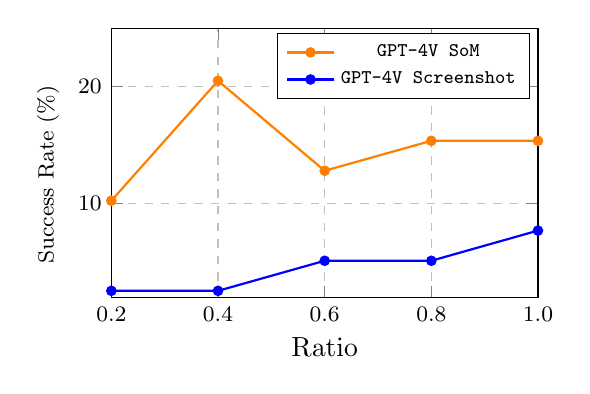
\begin{tikzpicture}
\begin{axis}[
    width=7cm, height=5cm,
    xlabel={Ratio},
    xlabel style={yshift=0.2ex},
    ylabel={Success Rate (\%)},
    ylabel near ticks,
    ylabel style={xshift=-1ex},
    grid=both,
    xmin=1, xmax=5,
    ymin=2, ymax=25,
    xtick={1, 2, 3, 4, 5},
    xticklabels={0.2, 0.4, 0.6, 0.8, 1.0},
     ylabel style={font=\footnotesize},
    xticklabel style={font=\footnotesize},
    yticklabel style={font=\footnotesize},
    ymajorgrids=true,
    grid style=dashed,
    legend style={
        at={(1,1)},
        anchor=south east,
        xshift=-1.0mm,
        yshift=-9.0mm,
        font=\scriptsize,
    },
]

% GPT-4V SoM
\addplot[
    color=orange,
    mark=*,
    mark size=1.5pt,thick
    ]
    coordinates {
    (1,10.26)(2,20.51)(3,12.82)(4,15.38)(5,15.38)
    };
    \addlegendentry{\texttt{GPT-4V SoM}}

% GPT-4V Screenshot
\addplot[
    color=blue,
    mark=*,
    mark size=1.5pt,thick
    ]
    coordinates {
    (1,2.56)(2,2.56)(3,5.13)(4,5.13)(5,7.71)
    };
    \addlegendentry{\texttt{GPT-4V Screenshot}}
    
\end{axis}
\end{tikzpicture}
\vspace{-5pt}
\caption{The effect of downsampling on the screenshot on performance with down-sampling ratios of 0.2, 0.4, 0.6 and 0.8 and run on a subset (10\%) of examples.}
\vspace{-10pt}
\label{fig:resolution_effect}
\end{wrapfigure}

Despite the significant progress in display technology (1080P, 2K, and 4K), most VLMs are still trained on data far below these resolutions. 
We select the screenshot-only input and SoM setting to test the method's performance under different screen input down-sampling ratios (i.e., 0.2, 0.4, 0.6 and 0.8 of the original resolution), to evaluate the impact of resolution changes on model recognition ability and accuracy.
The output coordinates of the model for the screenshot setting are still expected to align with the original resolution (\textit{i.e.}, 1080P).
The effects of varying input resolutions on performance are shown in Figure~\ref{fig:resolution_effect}. 
For inputs based on pure screenshots, it is observed that an increase in resolution directly correlates with enhanced performance. 
This issue may arise from the discrepancy between the resolution of the screenshot and the coordinates of the output.
However, the scenario slightly differs on SoM.
Interestingly, a reduction in resolution to 768$\times$432 (down-sampling ratio of 0.4) leads to an improvement 
in the agent's performance and further diminishing the resolution even more to a down-sampling ratio of 0.2 results in a noticeable decline in performance. 

\paragraph{Longer text-based trajectory history context improves performance, unlike screenshot-only history, but poses efficiency challenges}

\begin{wrapfigure}{l}{0.5\textwidth}
\vspace{-12pt}
    \centering
    \begin{minipage}[b]{0.5\textwidth}
        \includegraphics[width=\textwidth]{images/obs_length_distribution.pdf}
        \vspace{-10pt}
        \caption{
        The length distribution of a11y tree as observation from sampled trajectories.
        }
        \label{fig:obs_length_distribution}
        \vspace{5pt}
    \end{minipage}
    \begin{minipage}[b]{0.5\textwidth}
    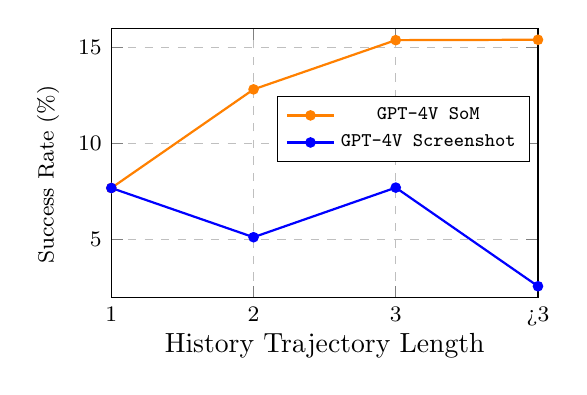
\begin{tikzpicture}
    \begin{axis}[
        width=7cm, height=5cm,
        xlabel={History Trajectory Length},
        xlabel style={yshift=1ex},
        ylabel={Success Rate (\%)},
        ylabel near ticks,
        ylabel style={xshift=-1ex},
        grid=both,
        xmin=1, xmax=4,
        ymin=2, ymax=16,
        xtick={1, 2, 3, 4},
        xticklabels={1, 2, 3, >3},
         ylabel style={font=\footnotesize},
        xticklabel style={font=\footnotesize},
        yticklabel style={font=\footnotesize},
        ymajorgrids=true,
        grid style=dashed,
        legend style={
            at={(1,1)},
            anchor=south east,
            xshift=-1.0mm,
            yshift=-17.0mm,
            font=\scriptsize,
        },
    ]
    
    % GPT-4V SoM
    \addplot[
        color=orange,
        mark=*,
        mark size=1.5pt,thick
        ]
        coordinates {
        (1,7.69)(2,12.82)(3,15.38)(4,15.40)
        };
        \addlegendentry{\texttt{GPT-4V SoM}}

    % GPT-4V Screenshot
    \addplot[
        color=blue,
        mark=*,
        mark size=1.5pt,thick
        ]
        coordinates {
        (1,7.69)(2,5.13)(3,7.71)(4,2.58)
        };
        \addlegendentry{\texttt{GPT-4V Screenshot}}
        
    \end{axis}
    \end{tikzpicture}
    \end{minipage}
    \vspace{-10pt}
    \caption{The effect of length of history on performance with the history encoding length of 1, 2, 3, and $>3$ and run on a subset (10\%) of examples.}
    \label{fig:history_effect}
    \vspace{-20pt}
\end{wrapfigure}

The main experiment revealed the decisive role of the a11y tree in performance within the current technological context. 
Even when we retain key attribute elements based on heuristic rules (keep nodes with tags of the document, item, button, heading, label, \textit{etc}.), LLMs still require a sufficiently large context to process this information effectively. 
To further understand this, we sample some a11y tree observations from \ours and conducted the statistical analysis, as shown in Figure~\ref{fig:obs_length_distribution}. 
The analysis indicates that a context length of 6000 is needed to accommodate about 90\% of cases for a single observation.
However, relying solely on current observations inherently leads to agents making repeated errors.
Therefore, we include current observations as well as past \texttt{N} rounds of observations and actions in the constructed prompts (see appendix for more details), to explore the impact on agent performance when \texttt{N} is set to 1, 2, 3, and all where we put as much context as we can.
The experimental results (as shown in Figure~\ref{fig:history_effect}) show the performance increase with more history context for SoM.
Future work on constructing models with enhanced capabilities for longer context support and understanding reasoning, improving model efficiency, and designing new agent architectures for efficient memory storage will have a significant impact on digital agents.

However, we also note that the inclusion of additional trajectory history does not enhance performance under the pure screenshot setting.
This suggests that contemporary advanced VLMs might not be as adept at extracting robust contextual information from images as they are from textual data. 
Strengthening this capability to harness information from images constitutes an important avenue for future enhancements.



\paragraph{VLM agents struggle with perturbation of position and size of application windows and irrelevant information}
\begin{wrapfigure}{l}{0.4\textwidth}

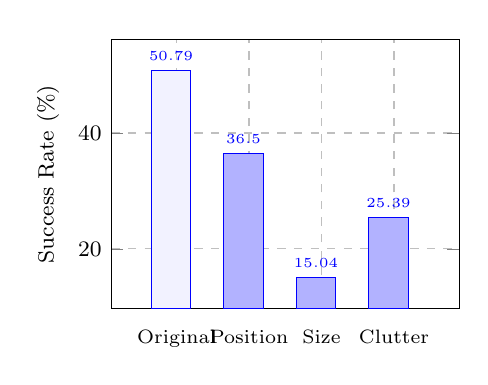
\begin{tikzpicture}
    \begin{axis}[
            ybar=3.8pt,
            enlargelimits=0.15,
            enlarge x limits=0.3,
            width=6cm, height=5cm,
            bar width=0.5cm,
            grid=both,
            grid style=dashed,
            every axis label={font=\footnotesize},
            tick label style={font=\footnotesize},
            legend style={at={(0.5,1.25), font=\tiny},
            anchor=north,legend columns=-1},
            xlabel style={font=\footnotesize},
            ylabel={Success Rate (\%)},
            ylabel style={font=\footnotesize,xshift=2.5em},
            ylabel near ticks,
            symbolic x coords={Original, Position, Size, Clutter},
            xtick=data,
            xlabel near ticks,
            xtick style={draw=none},
            ylabel style={font=\footnotesize},
            xticklabel style={font=\scriptsize},
            yticklabel style={font=\footnotesize},
            nodes near coords,
            nodes near coords align={vertical},
            nodes near coords style={font=\tiny}
        ]
        \addplot+[bar shift=-2pt, forget plot] coordinates {(Position, 36.50) (Size, 15.04) (Clutter, 25.39)};
        \addplot+[bar shift=-2pt, forget plot, fill=blue!5] coordinates {(Original,50.79)};
    \end{axis}
\end{tikzpicture}
    \vspace{-10pt}
    \caption{Decline in performance due to window perturbations.
    }
    \label{fig:ui_robustness}
    \vspace{-5pt}
\end{wrapfigure}

We continue to adopt the SoM setting and sample a subset of 28 tasks that agents relatively well perform (with a success rate of 50.79\%) in \ours.
At the beginning of each task, we introduce disturbances to the windows by 1) changing the 
\textit{position} of the window; 2) changing the \textit{size} of the window to the minimal; 
3) opening some irrelevant software and maximizing them to \textit{clutter} the screen.
This process generates several times more samples from the subset of tasks to observe their performance. 
We find current agents are not robust in handling all these changes, which leads to a performance drop to over 60\% to even 80\%.
Surprisingly, we find agents can switch the window to a certain degree but fail to maximize the window as an intermediate step and are stuck on other things. 
This suggests that while agents possess some capability to navigate between windows, they lack a comprehensive strategy for managing window states effectively.

\subsection{Performance across Different Operating Systems}
Another key challenge in building universal digital agents is ensuring that these agents can maintain efficient and consistent performance across different operating system environments. 
The differences between OS and their software ecosystems can significantly impact an agent's observation and action spaces, leading to performance uncertainties. 
Here, we explore and analyze the correlation between the success of agents in completing tasks on Windows after migrating from Ubuntu using examples from \ours.

\begin{wraptable}{r}{6cm}
\vspace{-0.1in}
\caption{Comparison of model performance and correlation across operating systems.}  
\centering
\resizebox{1.0\linewidth}{!}{%
\begin{tabular}{@{}lcc@{}}
\toprule
OS & SR (\%) & \small{Correlation Coefficient} \\ \midrule
Ubuntu           & 4.88               & \multirow{2}{*}{0.7}  \\
Windows          & 2.55               &                        \\ \bottomrule
\end{tabular}
}
\vspace{-0.1in}
\label{tab:os_performance}
\end{wraptable}

We enhance the functionality of the \ours environment to support setting up initial experiment states, final evaluations, and obtaining observations such as the a11y tree and screenshots in Windows OS.
Additionally, we have made example-wise fine-tuning modifications to the existing subset in \ours for migration to Windows. 
We conduct evaluations using the GPT-4V screenshot-only method and present the correlation of performance across the two operating systems. 
As shown in Tab.~\ref{tab:os_performance}, the model's performance on Ubuntu and Windows is 4.88\% and 2.55\%, respectively, with a correlation coefficient of 0.7, despite the differences in their observation spaces.
This implies that insights and methodologies developed within the \ours framework can be effectively transferred to Windows environments with a high degree of reliability.

\subsection{Qualitative Analysis}
\label{qualitative_analysis}
In this section we highlight representative examples of success, failure, and surprising outcomes, alongside a comparative study between GPT-4V and Claude-3 agents, to elucidate the unique challenges and insights our environment introduces. 
See App.~\ref{appendix:qualitative_analysis} for more details.

\paragraph{Success and failure cases}
We find agents, particularly based on GPT-4V, can successfully solve tasks that involve complex problem-solving or creative thinking, showcasing the advanced understanding and processing capabilities of the model already.
One successful task is shown in the first row of Figure~\ref{fig:success_example}. 
The agent is requested to extract subtitle files from the video stream and save them locally. 
The agent first divides the screen into two parts, with the VLC application window on the left and the terminal window open on the right, and uses the ffmpeg command twice. 
The first use removes the subtitles embedded in the original video, and the second use saves the extracted subtitles locally.

\begin{figure}[htbp]
    \vspace{-5pt}
    \centering
    \includegraphics[width=\linewidth]{images/qualititive_analysis/success_example.pdf}
    \caption{
    The agent successfully understood the complex task instructions, extracted the subtitle file from the video, and generated a pure video without embedded subtitles.
    }
    \vspace{-5pt}
    \label{fig:success_example}
\end{figure}

Despite the successes, there are notable failures that highlight the limitations of current models. In the task of ``center-aligning the title of the document'' (Fig.~\ref{fig:failure_human_agent} line 1), the agent fails to ground the relatively simple requirement of ``center alignment of texts'', performing many useless actions such as selecting irrelevant words, opening irrelevant menus, \textit{etc}.

Moreover, we find that the agent lacks prior knowledge in using software, performing poorly in many specialized tasks (as shown in Fig.~\ref{fig:model_lack_knowledge}, with GIMP, LibreOffice Calc, and Chrome selected). 
Taking GIMP as an example, for the instruction ``reduce brightness'' the agent does not know which menu in the toolbar is for brightness adjustment and instead randomly tries until exhausting the maximum number of steps.


\paragraph{Common errors by GPT-4V agents}
Among the 550 failed examples from different settings in our sample, more than 75\% exist \textit{mouse click inaccuracies}, which is the most common error. 
The agent fails to click the correct coordinates despite planning detailed and accurate steps in their code comments, indicating strong planning but weak execution capabilities. 
Mouse click inaccuracies lead to two other frequent errors: 
\textit{repetitive clicks} and \textit{environmental noise dilemma}. 
Repetitive clicks occur when the agent repeatedly misclicks, adjusts, and fails, consuming too many steps. 
Environmental noise arises from clicking unintended objects, causing pop-ups, or opening unrelated applications. 
Due to a lack of prior knowledge about most professional software, it falls into a mismatch dilemma between the actions taken and the current state, and don't know how to get back to normal.
Moreover, the agent lacks basic human-like cognition of web pages, such as not closing pop-ups in real-world web pages or being attracted by advertisement content, which affects its original correct judgment. 
Failures also arise from \textit{misinterpretation of instructions} and \textit{visual oversight}, highlighting the need for improvement in language and visual processing. 
See App.~\ref{appendix:common_errors} for the specific execution process.

\begin{figure}[htbp]
    \centering
    \vspace{-5pt}
    \includegraphics[width=\linewidth]{images/qualititive_analysis/failure_human_agent.pdf}
    \caption{
    Screenshots of the three examples mentioned in the quality analysis. 
    The first line is an example of GPT-4V failing at a very simple task, the second line is one example where agents face more difficulty than humans, and the third line is one example that is more difficult for humans than for agents.
    }
    \vspace{-10pt}
    \label{fig:failure_human_agent}
\end{figure}


\paragraph{Discrepancies in task difficulty between agent and human}
We identify notable disparities in the perceived difficulty of tasks between humans and AI agents. Tasks that are intuitively simple for humans often present substantial challenges to agents, and conversely, tasks that humans find demanding can be more straightforward for agents to execute.
You can find more details in Fig.~\ref{fig:human_agent_supplement} and App.~\ref{appendix:human_vs_agent}.

\paragraph{Tasks where humans outperform agents
} These tasks mainly involve text-based and design-related work, such as ``bold the font on this slide and add notes'' or ``erase all the highlighted marks in this document'' (Fig.~\ref{fig:failure_human_agent} Line 2). 
Since the Internet lacks such fine-grained data as the software execution process, the agent also lacks the corresponding training process, so its grounding ability is not good enough.
The lack of understanding of GUI logic also causes poor performance on operations like selecting and scrolling.

\paragraph{Tasks where agents outperform humans} Tasks that the agent considers simple but humans find difficult are concentrated in ``code solvability tasks'', such as ``monitor the system CPU for 30s and output the results'' and ``force close a process''. 
These tasks require little or no GUI interaction and can be completed by executing complex codes and instructions. 
It's worth noting that completing through code sometimes mismatches with human instructions. 
In the task "use GIMP to cut out the 2s to 4s part of a video,(Fig.~\ref{fig:failure_human_agent} Line 3)" the agent used ``ffmpeg'' command to complete the video cropping, ignoring the ``use GIMP'' requirement in the instructions.

Surprisingly, we discovered that agents are as prone to inefficiency in mechanically repetitive tasks, such as copying, pasting, and batch editing of Excel sheets, as humans. 
Humans frequently commit careless errors during execution. 
The shortcomings in agents stem either from the absence of an API or from insufficient training data related to the API, hindering their ability to efficiently process tasks in batches. 
Furthermore, sluggish response times can cause tasks to either time out or surpass the maximum allowed steps.

\paragraph{Comparative analysis: Claude-3 vs. GPT-4V}
Although Claude outperforms GPT-4 in many benchmarks such as GSM8K, HumanEval, \textit{etc}., in our main experiment, we find that Claude has an average lower accuracy rate compared to GPT-4V by 2.84\% to 7.76\%. 
We find that Claude can provide satisfactory high-level solutions, but its grounding ability contains hallucinations in detail.
For instance, Claude would interpret double-clicking a file as selecting it instead of opening it, treat column B in LibreOffice Calc software as column C, and enter text in the VS Code text replacement box without clicking on global replace. 
This shows that Claude can align well with human planning in problem-solving, but lacks excellent grounding ability when it comes to execution. Details can be seen in Fig.~\ref{fig:claude_error} and App.~\ref{appendix:claude3}.
